
\chapter{Grundlagen}


\section{ABB}

ABB ist ein global f\"{u}hrender Hersteller und Serviceanbieter in der Energie- und Automatisierungstechnik mit Hauptsitz in Z\"{u}rich.
Der internationale Konzern entstand 1988 aus der Fusion des schwedischen Unternehmens \ac{ASEA} und der schweizerischen Firma \ac{BBC}. ABB besch\"{a}ftigt zurzeit \"{u}ber 132.000 Mitarbeiter in 100 L\"{a}ndern. Im Jahr 2016 wurde ein weltweiter Umsatz von 33,8 Mrd. USD und ein Nettogewinn von 2,1 Mrd erwirtschaftet.\footnote{Vgl. ABB Gesch\"{a}ftsbericht 2016} 
\linebreak



\begin{figure}[ht]
	\centering
	\makebox[\textwidth][c]{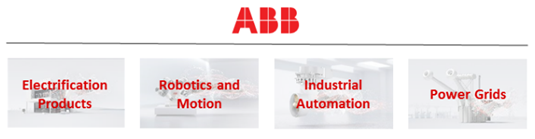
\includegraphics[width=1\textwidth]{img/ABB-Div.png}}%
	
	\caption{Divisionen von ABB}
	\label{fig1}
	
\end{figure}

Das Produktportfolio von ABB gliedert sich in vier Divisionen auf: Division Electrification, Robotics and Motion, Industrial Automation und Power Grids. Diese Aufteilung ist auch in Abbildung \ref{fig1} zu sehen.


\section{SAP}



\ac{ERP} Standardsoftware SAP R/3, welche bei ABB zum Einsatz kommt. Eine Standardsoftware ist ein Produkt welches die allgemeinen Anforderungen des Nutzers, in diesem Fall ABB, erfüllt und bei speziellen Anforderungen individuell angepasst werden kann. Die Firma SAP SE bietet verschiedene Modulare Lösungen an, welche einzeln genutzt werden können. Beispiele sind hierfür das \ac{SD}-, \ac{FI}-, \ac{MM}- und \ac{HR}-Modul. \\ 

SAP SE hat eigens für ihr \ac{ERP}-System die Programmiersprache \ac{ABAP} entwickelt. Mit Hilfe dieser w



\section{Dokumente im SAP}
\subsection{Smart Forms}

Um die Dokumentenerstellung im SAP zu vereinfachen wird seit dem 4.6C Release von SAP Smart Forms angeboten. Diese neue Technologie sollte vor allem dafür sorgen, dass für die neu Entwicklung und Anpassung von Dokumenten im SAP keine Experten mehr von Nöten sind.


\subsection{Adobe PDF}




\section{Langzeit-Lieferantenerklärung}

 Lieferantenerklärungen (LE) sind Dokumente, welche bei einer Lieferung Auskunft bezüglich der Präferenzursprungseigenschaft beinhaltender Waren gibt. Diese Angaben werden bei verschiedenen Zollprozessen benötigt. Grundsätzlich wird die Lieferantenerklärung bei Warenbewegungen innerhalb der \ac{EU} verwendet. Die \ac{LLE}, welche als Beispiel-Dokument für diese Arbeit benutzt wird, ist eine einmalige Erklärung welche für gleiche Lieferungen über einen maximalen Zeitraum von 2 Jahren gilt.\footcite{ZOLL.2017} 2016 erstellte ABB alleine in Deutschland dieses Dokument 1800 mal.\footnote{Nach Internen Auswertungen} Text und Aufbau der \ac{LLE} sind vorgegeben. Dementsprechend wird in der folgenden Arbeit nur auf die technische Umsetzung selbigen eingegangen.
